\documentclass[11pt]{letter}
\usepackage{amsmath,amsthm,amssymb,amscd}
\usepackage{graphicx}
\usepackage{epstopdf}
\usepackage{multirow}
\usepackage{hhline}
\usepackage{cleveref}
\usepackage{xcolor}
\usepackage{tikz}
\usepackage{comment}
\usepackage{mathpazo}
\usepackage[utf8]{inputenc}
\usepackage[margin=1in]{geometry}
\usepackage{setspace}

\onehalfspacing

\newcommand\qa{\begin{center}\line(1,0){250}\end{center}\begin{quote}\begin{em}}
\newcommand\qb{\end{em}\begin{center}\line(1,0){250}\end{center}\end{quote}}
\newcommand{\bx}{\boldsymbol {x}}
\newcommand{\bs}{\boldsymbol {s}}
\newcommand{\bt}{\boldsymbol {t}}
\newcommand{\bc}{\boldsymbol {c}}
\newcommand{\eps}{\varepsilon}
\newcommand{\todo}[1]{ {\color{red} #1 }}

\begin{document}


\signature{Jeremy Hoskins\\
Manas Rachh}

\address{Jeremy Hoskins (Yale University)\\
jeremy.hoskins@yale.edu\\
\vspace{.02in}\\
Manas Rachh (Flatiron Institute)\\
mrachh@flatironinstitute.org}


\begin{letter}{Editorial Office\\
Journal of Computational Physics - X}

\opening{Dear Editor:}

The following document contains a response to the comments made by the
reviewers after reading our manuscript \emph{On the discretization of Laplace's equation with Neumann boundary conditions on polygonal domains}.

Below are the reviewers' reports indented and in italics, interlaced with
our responses.

\qa
Reviewer \#1:
This manuscript extends a recent line of work on handling the singularities in the density of the standard boundary integral equation formulation of Laplace's equation that arise at the corners of polygonal domains, through the use of specialized, high-order quadratures, which are computed using analytic expansions of the density. Previous work in this direction has difficulties directly applying this strategy to Neumann problems, since the singularities are significantly worse here than in the Dirichlet case. The current work makes the incredibly interesting observation that one can instead use the adjoint of a discretization to the Dirichlet problem to obtain a solution that is accurate in a weak sense. Furthermore, pointwise accuracy in a region arbitrarily close to a corner can be obtained through a novel local refinement process. The relevant theory for justifying both that this approach yields a density that can be accurately interpolated away from the corners and that the refinement process can be done in a completely local manner is developed. Furthermore, the approach is illustrated through exceptionally thorough and impressive numerical results.

In my opinion, this paper certainly should be published, due to the very high quality of the work and good presentation. However, the manuscript in its current state is missing a few details that I believe are of crucial interest to potential readers and is confusing in a few places. I suspect that a couple of these missing details are present elsewhere in the literature, but I still believe that it would be valuable to include them here for the purpose of producing a relatively self-contained work. Furthermore, there are several suspected typos and notational inconsistencies that should be fixed to maximize readability. When these are resolved, I think this will be a very strong paper.

Remarks on content and readability

1) p. 2. The last sentence of the first paragraph mentions that the disadvantage of compression-based approaches to quadrature is cost in 3D. Given that these approaches have already been used in 3D problems, unlike the work in the current paper, I think that as a minimum there should be a couple of brief remarks somewhere about how the method here would extend and scale to 3D.

\qb

The discussion about the disadvantage of compression-based approaches in 3D has been removed and a discussion in the second last paragraph about generalizations to 3D has been added.

\qa
2) p. 6. On a first reading, Theorem 6 is not easy to digest. Could you add a few comments to provide some intuition for this result, and also a comment on the connection of the result on an open wedge to the case of polygons? Do we expect the expansions to be exactly the same?

\qb

The notation in Theorem 6 has been cleaned up and a remark has been added afterward discussing the connection between the problem on the polygon and the problem on the wedge.


\qa
3) p. 8. I think it is extremely important to explicitly discuss how large we expect K to be in section 4.1.1, especially how it relates to the accuracy a user might desire. I realize the relevant information is likely in [14], but it is of sufficient importance to the current work to make this clear by either stating a result or computational experience.

\qb

The value of K used in our experiments has been stated explicitly.

\qa
4) p. 11. The theory as developed considers only the exterior Neumann problem. I'm guessing a similar duality relationship holds with the interior Neumann problem and the exterior Dirichlet problem, and the procedure carries over straightforwardly (indeed, you consider an interior Neumann problem in the numerical results). For the sake of completeness, could you add a brief remark on whether or not the procedure is exactly the same for the interior Neumann problem, and state if there are any special considerations that are different from the exterior Neumann case?

\qb

We thank the referee for pointing this out. A comment has been added discussing the interior Neumann problem.

\qa
5) p. 13. I find the choice of notation in Theorem 8 to be very poor. In particular $A_{0}$ and $f_{0}$ are
used right above in (56) to denote the local problem after the corner has been refined ($A_{0}$ is of size
$P + 2M \times P + 2M$). Then in the statement of the theorem, these variables are used to denote the
analogous variables on just the corner panel of the unrefined problem ($A_{0}$ is of size $P \times P$ ), and then
in the proof of the result these variables are used to refer to the original corner panel as well as the
adjacent panels ($A_{0}$ is of size $P + 2M \times P + 2M$ ). Also, I am not sure why $f_{0}$ is not underlined, since it is a vector. Could you please fix this notation?

\qb

The theorem has been eliminated in favor of a remark, and the corresponding notation has been cleaned up.

\qa
6) p. 19. In the same vein as comment 3, I find the absence of any information on conditioning to be a bit startling, since one of the main appeals of working with boundary integral equations is the ability
to form well-conditioned discretizations. Again, I am aware that this falls squarely into the scope of existing work (again, probably [14]), but find this also sufficiently important to at least summarize in the current work.

\qb
We have included a remark to point out that the conditioning for the solution of Neumann problem is inherited from its corresponding Dirichlet discretization. (see remark 5.3)

As noted, with our approach, the conditioning of the discrete system for the Neumann problem inherits the properties of the corresponding Dirichlet discretization. The conditioning of using this approach as expected is independent of the number of points used in the discretization. However, the physical conditioning of the problem itself is fairly complicated owing to the presence of continuous spectra on various intervals whose sizes depend on the angles formed at the corners. This is reflected in any Dirichlet or Neumann discretization for regions with corners and falls outside the scope of this work. For the triangle example, we have included a plot of the spectrum of the operator here for reference. We also plot the spectrum of the discretized operator based on a dyadic mesh at the corner.
\begin{center}
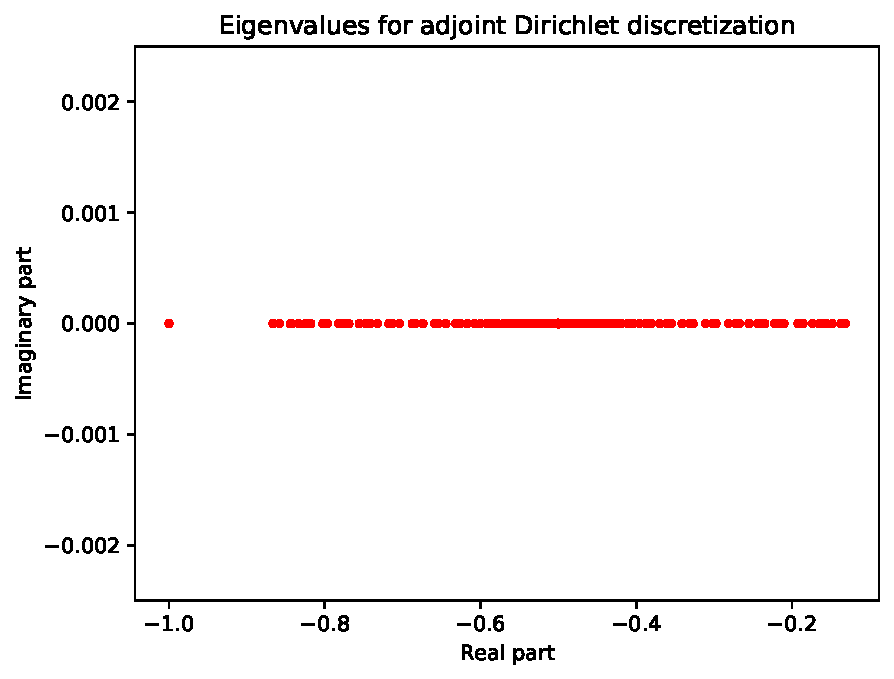
\includegraphics[width=0.4\linewidth]{sp-eigs-plot.pdf}
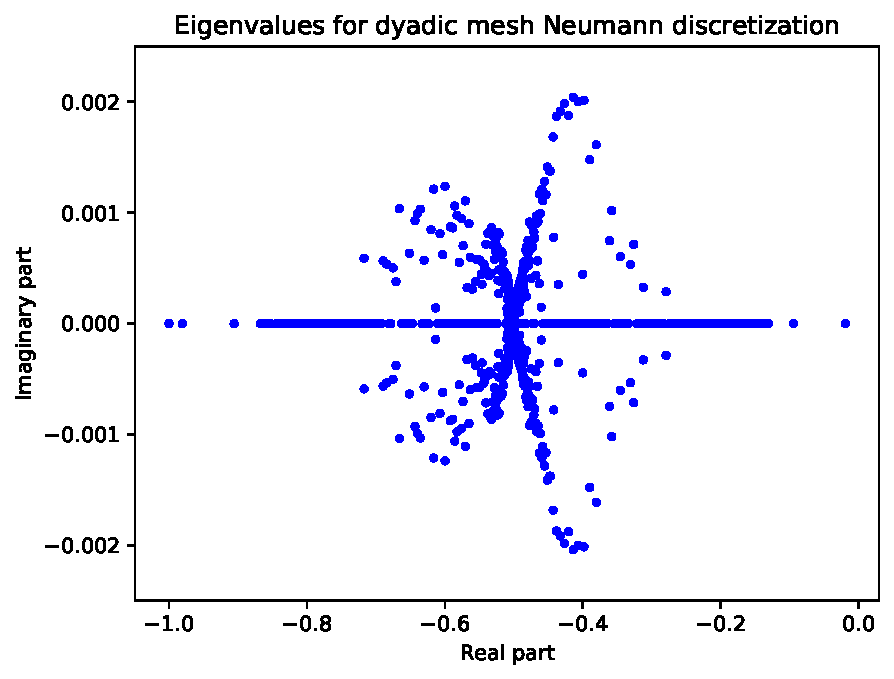
\includegraphics[width=0.4\linewidth]{ref-eigs-plot.pdf}
\end{center}


Similar plots for the singular values of the operators for Dirichlet problem for Laplace and Stokes equations have already been reported in [1] and we feel that it would take away from the main point of the paper.

1. K.~Serkh, V.~Rokhlin, On the solution of elliptic partial differential
  equations on regions with corners, Journal of Computational Physics 305
  (2016) 150--171.

\qa
7) p. 19. Even for a problem with 22k dofs, 105 iterations of a Krylov method seems like a lot, especially if the problem is well-conditioned. I can't help but wonder if this is an artifact of the fact that your FMM tolerance is the same as your iterative method tolerance. If you set the latter to 1e-14 or 1e-13, does the number of iterations decrease drastically?

\qb
We use a version of GMRES which does not suffer from stagnation at low thresholds and an FMM whose tolerance was set to $5 \times 10^{-16}$. The number of iterations do not reduce drastically if we increase the iteration count. We attach here a plot of the relative residual as a function of iteration number. 
\begin{center}
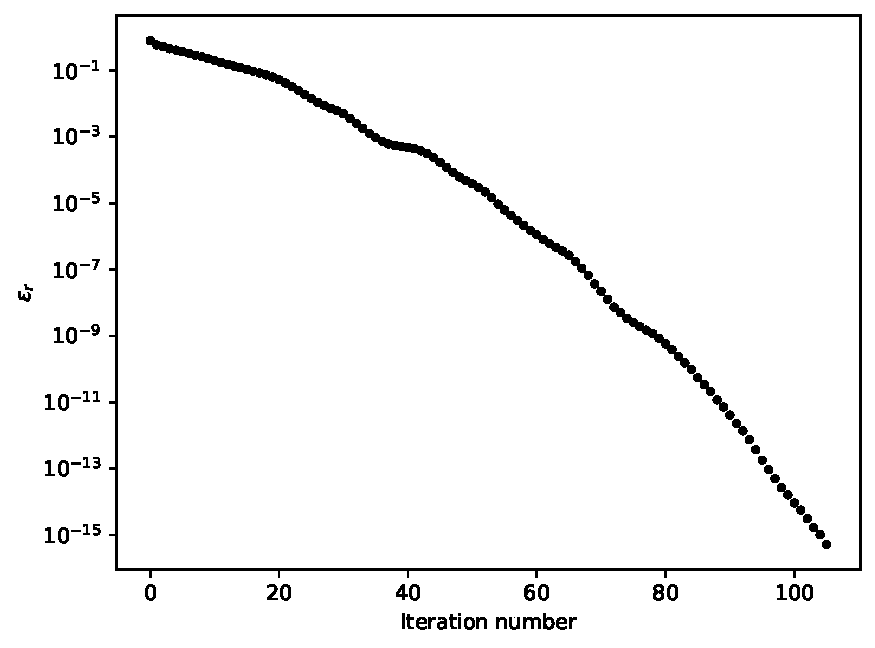
\includegraphics[width=0.7\linewidth]{lap-iter-count-wheel.pdf}
\end{center}

Our boundary data has randomly generated charge strengths and sources. For a new run, the original discretization requires $106$ iterations for the Neumann problem. The iteration count for the corresponding adjoint Dirichlet problem is $83$, and iteration count on doubling the number of points in our existing discretization is $106$. 

\qa
8) 
p. 21-22. I find the content of Appendix B difficult to understand for a number of reasons. The motivation for such a result is clear, but I'm not sure I totally understand the conclusion. In particular, you want to show that using the adjoint discretization one can interpolate the density on a panel far from the corner. That makes sense. Your approach to showing this is to use the relation (B.1) to find another equivalent integral equation, which you then show can be solved using existing information accurately.
Is the claim that to actually interpolate the density on such a panel, one would need to solve another Dirichlet problem, and it does NOT suffice to just interpolate the value of $\sigma$ obtained on the GL nodes when solving the original problem? Please clarify this point.

There are these other issues I'm having with it:
(a) On your assumptions about the discretization, 1 and 3 have an easy-to-understand interpretation. It's unclear to me what 2 is really assuming about the discretization, given that it seems to mostly to be introducing notation. Of course, I can imagine conditions where $\rho_{0}$ is less than the width of some panels, but is there some deeper restriction?
(b) Your assumption that $\rho_{0}>1$ and your later statement that the rate at which a polynomial interpolant will converge is $C \rho_{0}^{M}$ is a bit awkward, since these choices are specific for a function
on an interval of length 2.
(c) The second paragraph on p. 22 is very unclear to me. I don't even understand the first sentence as to why k(s,t) would be identically 0 on the same segment as $\gamma([s1,s2])$, or what is really even meant by segment here. Furthermore, it is mentioned that k(s, t) when considered as a function of $t \in \mathbb{C}$ has a singularity at $\gamma(s)$. Given the current setup wouldn't the singularity be at s? I would recommend rewriting this entire paragraph to be more transparent.

\qb
Thank you for bringing this to our notice. The section as written was confusing and we have rewritten the section completely to address all of the concerns above and feel that the readability now is significantly improved. We have eliminated the assumptions on the geometry completely as it can be confusing and rather reduced it to an error estimate of a solution to a Dirichlet problem using the same grid. The purpose of our approach is to show that a good Dirichlet discretization of the corner problem can be reutilized to obtain a discretization of the Neumann problem.
\qa
Small fixes and typos:

\qb
We thank the referee for pointing out these typos and small fixes!



\qa
Reviewer \#4:
This article is not suitable for JCP. Most of it is Theorem, Lemma, Proposition, Remark. Journal of Computational Physics focuses on computational aspects of physical problems and contributions in mathematical and numerical modeling, rather than numerical analysis. This paper should be submitted to SIAM NUM ANALYS., or IMA J. NUM. ANAL., or Numerische Mathematik.


\qb
The solution of Laplace's equation in complicated domains is a classical problem in computational physics and has many applications such as electrostatics, fluid flow, diffusion, and magnetohydrodynamics to name a few.  We have significantly reduced the use of theorems and definitions to summarize classical results and standard definitions.  Here are a few other examples of papers in JCP which we believe are written in a similar style.


\begin{enumerate}
\item G. Widmer, R. Hiptmair, C. Schwab, Sparse adaptive finite elements for radiative transfer, Journal of Computational Physics 227 (2008) 6071-6105. 
\item K. Serkh, V. Rokhlin, On the solution of elliptic partial differential equations on regions with corners, Journal of Computational Physics 305 (2016) 150-171.
\item C. Jerez-Hanckes, C. Peres-Arancibia, C. Turc, Multitrace/single trace fomulations and domain decomposition methods for the solution of Helmholtz transmission problems for bounded composite scatterers, Journal of Computational Physics 350 (2017) 343-360. 
\end{enumerate}

\qa

The scope of the article completely misses an entire arena of literature in the field, the unified transform (Fokas) method that has attacked the problem at hand in a much cleaner and nicer way in only 12 lines of code. It does not require a discretization with 22,240 points. See the work by Dr. Anthony Charles Lewis Ashton, Matthew J. Colbrook, and Natasha Flyer.

\qb

The unified transform method while handles the solution of Laplace's equation on simple polygons, does not scale in performance for larger problems like the ones presented in the paper. The "broken wheel" region for which $22,240$ discretization nodes are used, has $107$
corners and edges, thereby just requiring approximately $200$ nodes per edge for discretization. Moreover, our method is accelerated with simple modifications to the standard FMMs and thereby able to solve such problems in $O(N)$ CPU time, where $N$ is the number of degrees of freedom required to discretize the problem. We believe that Fokas' method wouldn't be competitive in performance when compared to our method on complicated geometries (105 iterations in 15 secs to obtain 13 digits of accuracy in the computed solution and plotting the solution at 250000 points in 6.5 secs on a single CPU core).
Moreover, our method also extends to discretizations of the Helmholtz problem (for any complex wave number in the first quadrant) and we are currently preparing a manuscript which describes the discretization procedure for both Dirichlet and Neumann boundary value problems. 
\qa

The method does the simplest of problems, Laplace on a convex domain, that was attacked much earlier and neater in 2001/2003 by Fokas. This paper does not show non-convex polygonal domains or Helmholtz or modified Helmholtz.

\qb

As stated above, the approach does not scale well for large complicated problems. Moreover, our example for the solution in the exterior of the "broken wheel" geometry is emphatically non-convex and we believe is suitably complicated as well. 




We thank the reviewers for their careful reads of our manuscript, and comments 
which have helped significantly improve the quality of the manuscript.
We hope that our revised manuscript based on their suggestions is now
suitable for publication in JCP-X.


\closing{Sincerely,}

\ps


\end{letter}

\end{document}
